\documentclass[12pt]{article}
\usepackage{amsmath,amssymb,amsthm}
\usepackage[utf8]{inputenc}
\usepackage{graphicx}
\usepackage{subcaption}
\usepackage{longtable}
\author{Mircea Grecu and John E. Yorks}
\title{Response to Reviewers}
\date{}
\begin{document}
\maketitle


\noindent \textbf{Reviewer 1:}
\noindent\textit{ \textbf{General Summary:}
This a well-written paper that fits within the scope of Journal of Atmospheric and 
Oceanic Technology and presents important and exciting results. The authors construct
 profiles of ice clouds based on CloudSat observations and then simulate retrievals 
 based on the instruments of the planned AOS mission. There are, however, 
 a few important ways in which the paper could be strengthened. I recommend 
 publication after the following comments are addressed.}\\
\newline
 We thank the reviewer for their perspective and constructive suggestions. Our point by point response is 
 provided below.\\
\newline
\textit{\textbf{Major Comments:} 1) There are several large sources of uncertainty that will be present in real 
retrievals from AOS that are ignored in this paper. While there is certainly still 
value in such analysis, it needs to be made more clear in the paper that this is an 
idealized scenario, and there should be more discussion about the sources of 
uncertainty that will affect real-world retrievals. Several in particular stand 
out to me. For one, it appears that all of the simulated measurements have been 
created at the same resolution (presumably, the resolution of CloudSat). This
should be clarified, and the authors should discuss how the lidar, radar, and 
radiometer will all have different resolutions and how this might affect results. 
Second, the electromagnetic scattering properties assumed in this study are 
unlikely to perfectly match reality. Finally, it appears that no measurement 
uncertainty has been assumed. The last paragraph of the paper does briefly mention 
many of these uncertainties, but they need to be introduced earlier in the 
manuscript, and more details are needed about the specifics of how IMPACTS
will help mitigate them.}\\
\newline
We thank the reviewer for the uncertainty discussion. Yes, indeed the resolution of the simulated 
observations is that of the CloudSat, while the AOS instruments are expected to have different resolutions,
which might impact results. In the revised manuscript, we included statements to convey this aspect.
We agree that the assumed electromagnetic scattering properties assumed in the study although
reasonable may contain significant uncertainties.  We acknowledge this aspect in the revised manuscript 
as well. Regarding the measurement uncertainties, we account for them in the radar and radiometer simulations,
but only in a highly idealized way in the lidar simulations.  Specifically, we assume random errors with 0.0 mean
and 0.5dB standard deviation in the radar observations \cite{takahashi2008}, and a Noise-Equivalent-Delta-T (NEDT)
of 1K, which is a readily achievable level for modern satellite radiometer \cite{draper2015}. A complex 
model of space-borne lidar measurement uncertainties was developed in \cite{liu2006}, but its parameters are
difficult to reliably quantify from theoretical considerations based on instrument expectations alone. Instead, we
assume a simple multiplicative error model, with the multiplicative factor model as a log-normally distributed random
variable with 0.0 mean and 1.0 standard deviation, which result in observation uncertainties similar to those in
the radar observations. We acknowledge the limitations of this model in the manuscript.\\
\newline
\textit{2) You say in your abstract (and conclusion) that “the characteristics of 
the instruments e.g.,  frequencies, sensitivities, etc. are set based on the 
expected characteristics of the AOS mission.” However, the AOS mission 
specifications are still very much in flux. Therefore, for reproducibility, 
I suggest adding a table explicitly laying out the frequencies and 
sensitivities you assume for each instrument (radar, lidar, radiometer). 
Some of these (e.g., the radiometer frequencies) are mentioned in the text, 
but it would be nice to see it all in one place.}\\
\newline
We agree with the reviewer that, unfortunately, the AOS mission is still in flux. We added a table in the revised
manuscript to summarize the assumed instrument characteristics.\\
\newline
\textit{\textbf{Minor Comments}
Line 38: Where is 8.0 dBZ coming from? There should be a citation here, or it should be stated that this is 
an estimate of the radar’s expected sensitivity.}\\
\newline
This is an estimate of the radar’s expected sensitivity provided by Japan Aerospace Exploration Agency (JAXA), which the AOS International
partner contributing the Ku-band radar in the inclined orbit.\\
\newline
\textit{Lines 50-51: While your approach is justifiable and worthwhile, it is worth noting that your CloudSat IWC retrieval 
also makes numerous assumptions about ice cloud microphysical properties and structures (as laid out in Section 2a). 
So the problem is not entirely avoided by relying on “observations” instead of models, as the observations were of 
radar reflectivity, not of ice water contents or particle sizes.}\\
\newline
We agree. We do not consider CloudSat retrievals uncertainty or bias free, but we prefer them because
they are consistent with an observed vertical distribution of reflectivity at W-band. The vertical distributions of radar reflectivity
derived from satellite or ground-based observations are generally difficult to reproduce by model simulations. We added a statement 
to this effect in the revised manuscript.\\
\newline
\textit{Lines 65-67: This is fine, but it should be noted that in doing this, you are underestimating the true retrieval 
uncertainty. The particle distribution assumptions and electromagnetic scattering properties that you use in training 
the retrieval algorithm will almost certainly not perfectly reflect the actual size and shape distributions of ice 
particles around the globe.}\\
\newline
We agree. As described explained above, our  objective was to derive IWC distributions consistent with the observed vertical distribution of
CloudSat reflectivity, without implying that the resulting distributions are uncertainty or bias free.  To make the performance
assessment more realistic, in the revised version of the manuscript, we perturbed the $N_w$ value (which in the initial version was
parametrized as a function of height) used in the derivation of IWC as a function of observed CloudSat reflectivity by a random log-normally
distributed factor. This accounts for uncertainties in the PSDs (at least from the perspective of the normalized PSD framework) and 
makes the evaluation realistic. Nevertheless, as observed by the reviewer, the electromagnetic scattering properties are 
an additional source of uncertainty.  We included additional statements in the manuscript to describe $N_w$ perturbation approach and
discuss uncertainties in the electromagnetic scattering properties that are not quantified in the manuscript.\\ 
\newline
\textit{Lines 83-90 and Eq. (1): I looked over the Testud et al. (2001) paper, and could not find anything that directly
 supported this statement, or any equations that resembled Eq. (1). Please add further explanation, either here 
 or in an appendix, to help the reader follow your logic.}\\
\newline
We apologize for the confusion. Testud et al. (2001) only show that normalization by $N_w$ ($N_0^*$ in their notation) explains the variability
in Z-R relationships (fig. 9d). Ferreira et al. (2001) \cite{ferreira2001} make the more general statement that any two integrated rainfall parameters ($X$, $Y$) 
may be related through a power law of the form $X = m N_w^{(1-n)} X^n$, where $m$ and $n$ are constants almost independent of $N_w$. Delanoe et al. (2014)
 \cite{delanoe2014} show that the same relationship holds for ice PSDs. We added statements to this effect in the revised manuscript.\\
\newline
\textit{Figure 2: Neither the caption nor the text adequately explains what is being plotted in this figure. What does each 
individual point represent? The text says, “Figure 2 is a scatter plot representation of the class multiplicative 
coefficient ai as a function of relative height,” but if that were the case, I would expect there to be many more 
points on the scatter plot (i.e. 18 classes times a certain number of relative height levels, to yield hundreds of points).}\\
\newline
We apologize for the confusion.  The points in figure 2 were derived from a classification of the IWC profiles into 36 classes.  
We initially used 36 classes in the analysis, but
we reduced the number of classes to 18 to make the classification and the Ensemble Kalman Filter more robust.  
For consistency and simplicity in the revised manuscript we derive IWC-Z relationships 
for each CloudSat radar bin, with the bins indexed relative to the freezing level bin.  The relative height is now defined as the distance
between the height of the associated bin relative to the freezing level.  Results are quantitatively similar to those in the initial
submission, especially given that the differences between the current $a$/$N_w$ parameterization and the initial one are smaller than 
the random perturbations in $N_w$ that we introduced in the revised analysis to make the evaluation of the radar retrievals more realistic.\\
\newline
\textit{Lines 120-121: How is the data in Fig. 2 used to parameterize Nw as a function of height? Do you fit a line/curve to the 
data in Fig. 2? This needs to be clarified.}\\
\newline
Yes, we fit a line to determine the variation of $ln(a)$ as a function of height and then divide the slope by $(1-b)$ to get the variation of
$ln(N_w)$ as a function of height.\\
\newline
\textit{Figure 3: It would be helpful to add vertical lines to these plots to indicate the detection thresholds you are 
assuming for the radar (8 dBZ?) and lidar.}\\
\newline
We included vertical lines to indicate the detection thresholds.\\
\newline
\textit{Line 220: It is my understanding that an ensemble Kalman smoother assumes normal distributions. How much does it matter 
that IWC is not normally distributed in nature?}\\
\newline
Yes, the ensemble Kalman smoother assumes normal distributions.  We derive a Kalman gain, i.e. a matrix of type $\mathbf{Cov(X,Y) Cov(Y,Y)^{-1}}$, 
for every class, and although IWC is not normally distributed in nature, its conditional class distributions are not likely to be as skewed 
as the entire distribution.
This is most likely why the Kalman smoother produces rather accurate results when observations from all instruments is available.  
Nevertheless, from the theoretical perspective, the Kalman Smoother results are suboptimal given the non-Gaussian distribution of IWC.  This
does not necessarily mean that more accurate results may be derived in practice given the multitude of uncertainty factors that may
impact the results.\\
\newline
\textbf{Typos}\textit{Line 276: “wells” should be “well”}\\
\newline
Thank you for pointing that out. We corrected it in the revised version of the manuscript.\\
\newline
\textit{Line 308: Figure 8 should be Figure 9}\\
\newline
Thank you for pointing that out. We corrected it in the revised version of the manuscript.\\
\newline
\textit{Line 315: IWP should be IWC}\\
\newline
Thank you for pointing that out. We corrected it in the revised version of the manuscript.\\
\newline
\textit{Line 361: eliminate “out}\\
\newline
Thank you for pointing that out. We corrected it in the revised version of the manuscript.\\
\newline
\newline
%\newpage
\clearpage
\noindent \textbf{Reviewer 2:}
\newline \textit{The study investigates the synergy between observations from elastic backscatter lidar, Ku-band radar,
and sub-millimeter radiometer observations to retrieve ice concentrations. The topic is undoubtedly timely,
considering that AOS, NASA's upcoming satellite mission targeting remote sensing of the atmosphere,
is currently in its design phase. The methodology is sound, albeit slightly contrived. Methods and
results are presented in an accessible way.
Nonetheless, there are significant conceptual flaws in the study.}\\
\newline
We thank the reviewer for their perspective and constructive suggestions.\\
\newline
\noindent \textit{First of all, I can't entirely agree with the study's framing. Currently, 
the study investigates the synergies
achieved by adding lidar and radar observations to radiometer observations. 
However, since the active sensors will likely have a much narrower swath, 
combining these observations will only be possible at
a small part of the radiometer's swath. Given the significantly higher information 
content of the active observations, the more relevant question is: What is the 
benefit of including radiometer observations
when radar and lidar observations are available? Simply showing an added value 
from adding radar
and/or lidar observations to radiometer observations, which is the current main 
conclusion of the paper, is a trivial result.}\\
\newline
Although active observations are characterized by much narrower swaths and 
significantly worse temporal sampling, they are nevertheless crucial in process 
studies and the development and validation of products from radiometer-only
observations (\cite{stephens2008},\cite{sano2022},\cite{stubenrauch2021}).  The
particular combination of active and passive observations considered in this
study is justified by the current design of the AOS mission. Specifically,
the Ku-band radar is intended to enable accurate estimates of 
the convective precipitation.  Although it was originally envisioned that AOS would
deploy two Ku-band radars, one in an inclined orbit and one in a polar orbit, currently, only
the inclined orbit is expected to feature a Ku-band radar contributed by 
Japan Aerospace Exploration Agency - JAXA.  
The polar orbit radar will operate at higher-frequencies (Ka- or W-and) and 
have cloud-detecting capabilities (i.e. high-sensitivity), but
will not be able to provide direct observations of intense convective precipitation
due to attenuation. Moreover, the polar radar will have nadir-only capabilities,
while the inclined orbit radar will have a
swath of about 200 km.  Both the polar and inclined orbit radars will operate
in tandem with a lidar and a high-frequency radiometer.  We are interested
in the inclined orbit despite the significantly lower sensitivity of the 
Ku-band radar because the synergistic Ku-band radar, elastic lidar and radiometer
estimates of ice in anvil clouds can be studied jointly with various parameters
(i.e. precipitation intensity, vertical velocities, etc.) characterizing the
convective processes responsible for their creation.  Although 
the polar orbit instruments are likely to enable the derivation of more accurate 
synergistic ice estimates, their severely limited ability to quantify convection
makes synergistic ice retrievals from the combination of instruments studied in
this manuscript relevant to the problem of relating the strength of convection to
the horizontal extent of anvil clouds and their impact on climate \cite{hartmann2016}.
Although the improvement in the ice estimates due to the inclusion of radiometer 
observations may seem trivial, it is rather significant given that neither the
lidar nor the Ku-band radar can provide by themselves accurate and complete 
ice estimates, the lidar
due to attenuation and the radar due to its limited sensitivity and complex Particle
Size Distribution (PSD) variability. \\

\noindent \textit{Secondly, since the dependency of the multiplicative factor a is parametrized by relative height,
the authors essentially use a single-moment retrieval to determine the profile database upon
which they base their whole study. This approach will significantly underestimate the variability
in the retrieved PSDs. Pfreundschuh et al. 2020 show that this variability causes considerable
uncertainty in radar-only retrievals of ice water path and is one of the dimensions in which
radiometer observations can help to improve radar-only retrievals. Neglecting this variability
likely significantly overestimates the accuracy of the proposed retrievals.
Finally, I do not consider that the omission of seven ($!$) of the ten radiometer channels is justified,
given that the authors use the inability of the radiometer to reproduce the vertical distribution of
ice particles as a principal motivation for studying the synergy with active observations.}\\
\newline
We agree with the reviewer. The parametrization of the multiplicative factor $a$ is equivalent to a single-moment retrieval. In the revised
manuscript, to investigate the impact of variability in $N_w$, we randomly perturbed its parameterized value by a log-normally distributed
random variable with a standard deviation of 0.5. This was achieved by generating one-dimensional vectors of independent random variables
with a standard normal distribution and applying a Gaussian smoothing filter \cite{nixon2019}.  The filter size was chosen to be two CloudSat radar bins.
The initial standard deviation was scaled to result a standard deviation of 0.5 after smoothing, which is roughly consistent with the variability
in $N_w$ observed in real observations \cite{grecu2018}. \\
\newline 
Moreover, the revised manuscript includes all radiometer channels in the analysis. It should be noted though that the 183.31 and 321.15-GHz radiometer channels
are centered on water vapor absorption lines. The differences in the brightness temperatures observed by these channels are driven by the vertical distribution
of water vapor and have only indirect impact on the retrieval of ice.  This is particularly true for the simulated observations considered in this study, which
are not characterized by large variability in the vertical distribution of water vapor. Consequently, the inability of the radiometer to reproduce the vertical
distribution of ice particles is not likely related to the omission of these channels. We nevertheless included all channels in the retrievals, as the vertical
distribution of moisture is likely to be important in future versions of the methodology when more diverse environmental contexts are going to be considered.\\
\newline
\textit{\textbf{Major comments:}}
\textit{1. To address the first-mentioned issue above, the authors should include radar-only, lidar-only, and radar-lidar 
    retrieval in their analysis.}\\
\newline
We agree with the reviewer. The revised manuscript includes radar-only, lidar-only, and radar-lidar retrievals in the analysis.  Shown 
in Fig. \ref{fig:IWP_IWC} are density plots of single-instrument retrievals of IWP and IWC as a function of their reference values.
As apparent in the figure, retrievals from single active instruments exhibit significant deficiencies.  This is not surprising given that
the lidar observations are subject to significant attenuation, while a Ku-radar with the AOS specifications misses a significant fraction of
the ice clouds. A W-band cloud radar would do much better by itself, but as already stated in our response, a Ku-band radar in conjunction
with a backscatter lidar and a high-frequency radiometer is a very exciting prospect, as it enables the study of the relation between 
the strength of convection and the characteristics of associated anvil clouds. \\
%include figure
\begin{figure}
\centering
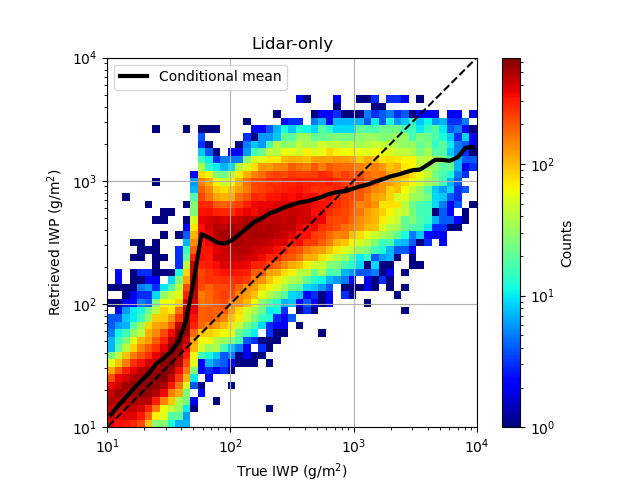
\includegraphics[width=.31\linewidth]{ResponseFigs/lidarOnly_IWP.png}
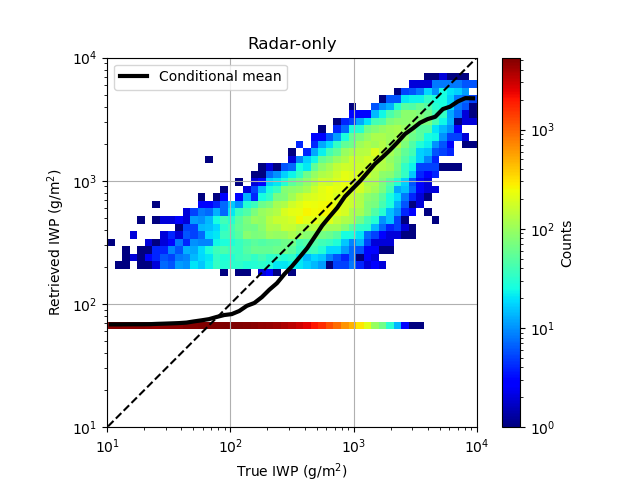
\includegraphics[width=.31\linewidth]{ResponseFigs/radarOnly_IWP.png}
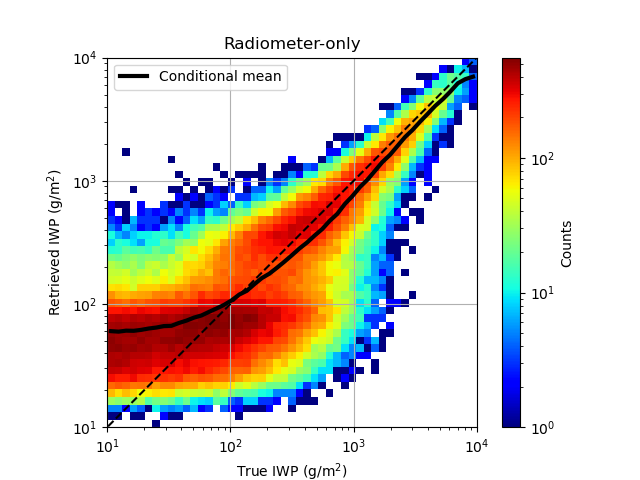
\includegraphics[width=.31\linewidth]{ResponseFigs/radiometer_IWP.png}
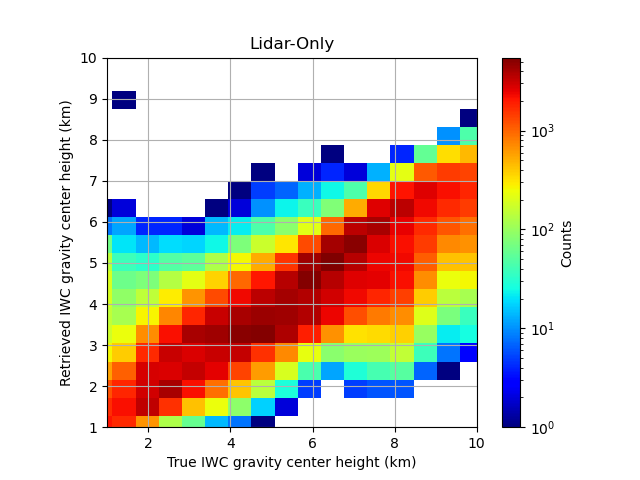
\includegraphics[width=.31\linewidth]{ResponseFigs/lidarOnly_GC.png}
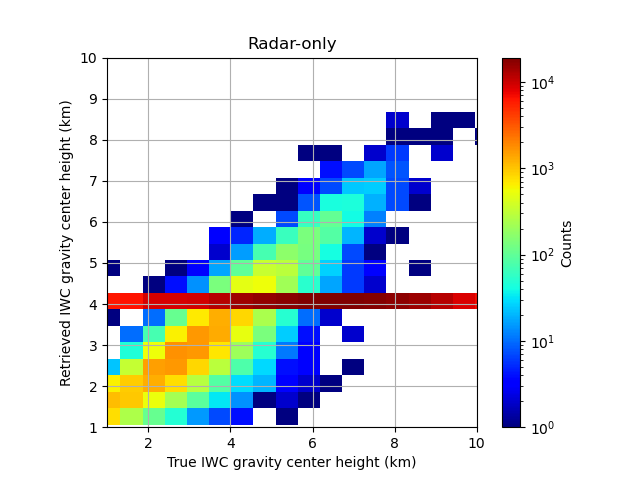
\includegraphics[width=.31\linewidth]{ResponseFigs/radarOnly_GC.png}
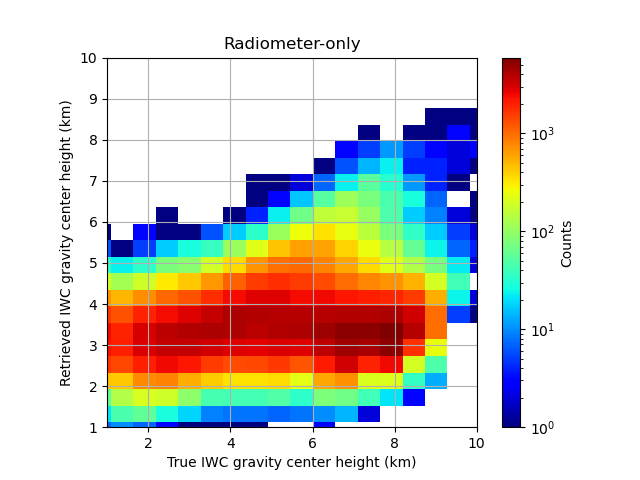
\includegraphics[width=.31\linewidth]{ResponseFigs/radiometer_GC.png}
\caption{Top Row: Density plots of IWP retrievals from lidar-only (left), radar-only (middle), and radiometer-only (right) observations as a function
of true IWP. Bottom Row: Same as in the top row but for IWC.}
\label{fig:IWP_IWC}
\end{figure}
    

\noindent
\textit{2. To improve the representation of microphysical variability in the retrieval, I suggest that the authors at 
    least randomize the parametrization of the multiplicative factor a in a way that covers the spread of the distribution 
    shown in Fig. 2.}\\
\newline
We agree with the reviewer. The revised manuscript includes a randomization of the parametrization of the multiplicative factor $a$.  Specifically,
we randomly perturb $N_w$ by multiplying its parameterized value with log-normally distributed
random variable with a standard deviation of 0.5.  As explained above, we use a Gaussian smoothing filter to impose a vertical auto-correlation in
$N_w$ similar to that observed in field experiments.\\
\newline
\textit{3. The authors should include all radiometer channels in their analysis.}\\
\newline
As explained above, we included all the radiometer channels in the revised version of the manuscript.\\
\newline
\textit{4. The introduction's title and first sentence mention "high ice clouds". However, the authors do not provide any 
    information on how the 'high ice clouds' are defined or what distinguishes them from regular ice clouds.}\\
\newline
In AOS terminology, high clouds are convectively generated high clouds \cite{braun2022}. Such clouds are the result of strong vertical mass transport 
from the lower troposphere and horizontal transport in the upper troposphere.  While preponderantly consisting of ice, high clouds may exhibit 
liquid phased hydrometeors. To make it clear upfront that we are not considering mixed-phase clouds in this study, we included ice in the title.
We included clarifying statements on the definition of high-clouds in the manuscript. \\
\newline
\textit{5. Although the authors state that the sensor characteristics are set based on the expected characteristics of the 
    AOS mission instruments, it is unclear whether thermal noise is included in the retrieval experiments. 
    The authors should mention this in the description of their methodology.}\\
\newline
No, we don't include thermal noise in the retrieval experiments.  We acknowledge the lack of an uncertainty component in 
the lidar model in section 2a.\\ 
\newline
\textit{\textbf{Minor comments}
    1. l. 29 - 31: Please provide more information on the planned or possible observation configuration of AOS, such as swath
     widths of the active instruments and the type of radiometer. The provided reference (Braun 2022) is missing, and I 
     could not find conclusive information on this online.}\\
\newline
We apologize for the missing reference.  We included a reference to an IEEE IGARS conference paper \cite{braun2022} that provides a brief description of the AOS mission.
The IEEE document is publicly available and provides a link to an additional AOS document (https://aos.gsfc.nasa.gov/docs/ACCP\_Science\_Narrative-2021.07.19.pdf). 
However, the swath widths of the active instruments are not explicitly specified, as architectures and instruments have been not finalized.  Nevertheless,
the Ku-band radar will be based on the GPM DPR radar and is expected to have a swath width of 245 km.  The elastic lidar will be in many respects 
similar to the CALIPSO/CALIOP lidar (https://calipso.cnes.fr/en/CALIPSO/lidar.htm) and will provide nadir observations,  while the radiometer is expected 
to have a swath of around 1000 km.\\
\newline
\textit{2. l. 83 -90: The results by Testud 2001 are for raindrops assuming Rayleigh scattering. It is not evident that this 
    is also generally true for ice particles.}\\
\newline
The impact of normalization on Z-IWC relationship is shown in \cite{delanoe2014}. Soft spheres were assumed and the Mie solution was used in \cite{delanoe2014}
to derive reflecitivities from observed Particle Size Distributions, but \cite{chase2021}  used more advanced backscattering models to calculate Z from
observed PSDs.  Their calculations are publicly available at https://github.com/dopplerchase/Chase\_et\_al\_2021\_NN and may be used to confirm the contraction
of the ($Z/N_w$,$IWC/N_w$) distribution to almost one-to-one relationships.  As explained in the manuscript, we use the self-similar Rayleigh-Gans approximation
to model the backscattering property of ice particles but get a normalization behavior similar to that anticipated by Testud et al. (2001),
shown in \cite{delanoe2014} and present in the \cite{chase2021} database.\\
\newline
\textit{3. l. 96: Please clarify: What do the authors mean by 'similarity'? Euclidean distance?}\\
\newline
Yes, the similarity is measured by the Euclidean distance.  We added a sentence to clarify this point.\\
\newline    
\textit{4. l. 112 and Fig. 2: Please clarify: Why are there 36 scatter points in Fig. 2.? How is the relative height value 
    of the scatter points derived?}\\
\newline
We initially started with 36 similarity classes and derived (through linear regressions in the log-log space) 
an IWC-Z relationship for each class. The points in Fig. 2 represent 
the coefficients $a$ as a function of the height of the class-average IWC peak for each class. We subsequently reduced the number of classes 
to 18 to make the classification and 
estimation process more robust. However, for consistency and simplicity in the revised manuscript we derive IWC-Z relationships 
for each CloudSat radar bins, with the bins indexed relative to the freezing level bin.  The relative height is now defined as the distance
between the height of the associated bin relative to the freezing level.  Results are quantitatively similar, especially given that the
differences between the current $a$/$N_w$ parameterization and the one used in the initial submission are smaller than the random
$N_w$ perturbations used in the analysis.\\
\newline
\textit{5. Fig. 2: Please add a line showing the parametrization used to derive the database.}\\
\newline
Thanks for the suggestion.  We added a line showing the parametrization used to derive the database.\\
\newline
\textit{6. l. 130: Please clarify: What is the assumed shape of the ice particles?}
The ice particles are aggregates of bullet rosettes, columnar crystals, and plates.  The aggregation model and 
other details are comprehensively described in \cite{hogan2014}. We added a sentence in the manuscript to clarify this point.\\
\newline
\textit{7. Fig. 3: Please clarify: Why is the distribution of radar reflectivities going to zero towards the freezing level? 
    What about precipitating clouds?}\\
\newline
We selected only CloudSat reflectivity profiles with no echo below the freezing level and the freezing level above ground.  
Profiles that satisfy this requirement include anvil clouds, whose quantification in relation to the convective process with which they are associated
is an AOS objective. We added a sentence in the manuscript to clarify this point.\\
\newline
\textit{8. l. 181 - 182: Please clarify: Do the authors mean surface emissivities?}\\
\newline
Yes, we mean surface emissivities.  We clarified this in the manuscript.\\
\newline
\textit{9. l. 198: Please provide more information on how the IWC and PSD parameters are estimated. If more than one moment
is estimated, the authors must use a priori assumptions to resolve the ambiguity in the retrievals.}\\
\newline
We derive the IWC as a function of CloudSat $Z$ and $N_w$.  The $N_w$ is given by the vertical parameterization and perturbed using the random model
described above and in the revised manuscript.  We added statements in the manuscript to clarify this point.\\
\newline
\textit{10. l. 203: I don't think that 200,000 profiles can be considered a large dataset by today's standards.}\\
\newline
We agree that 200,000 profiles is not a large dataset by today's standards.  However, these profiles are derived from a month of CloudSat observations.
Specifically, all CloudSat and 2C-ICE product files from June 2019 were processed, and only profiles with no echo below the freezing level
and the freezing level above ground were selected. The selection process significantly reduced the number of profiles. Nevertheless, there is sufficient
variability in the selected profiles to derive meaningful conclusions. We added statements in the manuscript to clarify this point.\\
\newline
\textit{11. Fig. 4: Please add lines marking the diagonal and conditional mean}\\
\newline
Thank you for the suggestion. We added the lines to the figure.\\
\newline   
\textit{12. Fig. 6: I think it would be valuable to check whether the classification step causes the multi-modal distribution 
    in the retrieval results. Please produce a version of Fig. 6 in which the 18 centers of gravity of the clusters 
    are marked using horizontal lines. The is, however, no need to include the figure in the manuscript if that doesn't lead
     to any conclusive results.}\\
\newline
Thank you for the suggestion.  We added the lines to the figure.\\
\newline  
\textit{\textbf{Typos}
    1. l. 323: Missing word}\\
\newline
Thank you for pointing this out.  We added the missing word.\\
\newline

\begin{longtable}[]{@{}llll@{}}

    Instrument & Frequency/Wavelength & Noise & Sensitivity \\
    \hline
    \endhead
    Lidar & 524 nm & LogNormal(0,1) & 1e-6 \\
    Radar & 13.8 GHz & 0.5dB & 8 dBZ \\
    Radiometer & 89 GHz & 1.0 K & N/A \\
    & 183.31+/-0.2 GHz & 1.0 K & N/A \\
    & 183.31+/-1.1 GHz & 1.0 K & N/A \\
    & 183.31+/-2.8 GHz & 1.0 K & N/A \\
    & 183.31+/-4.2 GHz & 1.0 K & N/A \\
    & 183.31+/-6.8 GHz & 1.0 K & N/A \\
    & 183.31+/-11 GHz & 1.0 K & N/A \\
    & 325.15+/-1.5 GHz & 1.0 K & N/A \\
    & 325.15+/-3.5 GHz & 1.0 K & N/A \\
    & 183.31+/-9.5 GHz & 1.0 K & N/A \\
   \hline 
    \end{longtable}

\begin{thebibliography}{999}

\bibitem{takahashi2008}
Takahashi N, Iguchi T. Characteristics of TRMM/PR system noise and their application to the rain detection algorithm. 
IEEE transactions on geoscience and remote sensing. 2008 May 16;46(6):1697-704.

\bibitem{draper2015}
Draper DW, Newell DA, Wentz FJ, Krimchansky S, Skofronick-Jackson GM. The global precipitation measurement (GPM) 
microwave imager (GMI): Instrument overview and early on-orbit performance. IEEE Journal of Selected Topics in 
Applied Earth Observations and Remote Sensing. 2015 Mar 2;8(7):3452-62.
\bibitem{liu2006}  
Liu Z, Hunt W, Vaughan M, Hostetler C, McGill M, Powell K, Winker D, and  Hu Y, 
Estimating random errors due to shot noise in backscatter lidar observations. 2006, Appl. Opt. 45, 4437-4447.

\bibitem{ferreira2001}
Ferreira, F., P. Amayenc, S. Oury, and J. Testud, 2001: Study and Tests of Improved Rain Estimates from the TRMM Precipitation Radar. 
J. Appl. Meteor. Climatol., 40, 1878–1899, https://doi.org/10.1175

  \bibitem{stephens2008}
  Stephens GL, Vane DG, Tanelli S, Im E, Durden S, Rokey M, Reinke D, Partain P, 
  Mace GG, Austin R, L'Ecuyer T. CloudSat mission: Performance and early science 
  after the first year of operation. 
  Journal of Geophysical Research: Atmospheres. 2008 Apr 27;113(D8). 

  \bibitem{sano2022}
  Sanò P, Casella D, Camplani A, D’Adderio LP, Panegrossi G. A Machine Learning
  Snowfall Retrieval Algorithm for ATMS. Remote Sensing. 
  2022 Mar 18;14(6):1467.

  \bibitem{stubenrauch2021}
  Stubenrauch CJ, Caria G, Protopapadaki SE, Hemmer F. 3D radiative heating of 
  tropical upper tropospheric cloud systems derived from synergistic A-Train 
  observations and machine learning. 
  Atmospheric Chemistry and Physics. 2021 Jan 26;21(2):1015-34.

  \bibitem{hartmann2016}
  Hartmann DL. Tropical anvil clouds and climate sensitivity. 
  Proceedings of the National Academy of Sciences. 2016 Aug 9;113(32):8897-9.

  \bibitem{braun2022}
  S. A. Braun, J. Yorks, T. Thorsen, D. Cecil and D. Kirschbaum, 
  NASA'S Earth System Observatory-Atmosphere Observing System, 
  IGARSS 2022 - 2022 IEEE International Geoscience and Remote Sensing Symposium, 
  Kuala Lumpur, 
  Malaysia. 2022, pp. 7391-7393, doi: 10.1109/IGARSS46834.2022.9884029.
  
  \bibitem{nixon2019}
  Nixon, M. and Aguado, A., Feature extraction and image processing for computer vision. 2019, Academic press.

  \bibitem{grecu2018}
  Grecu M, Tian L, Heymsfield GM, Tokay A, Olson WS, Heymsfield AJ, Bansemer A. Nonparametric methodology to estimate precipitating ice from multiple-frequency radar reflectivity observations. Journal of Applied Meteorology and Climatology. 2018 Nov;57(11):2605-22.

  \bibitem{delanoe2014}
  Delanoë, J. M. E., Heymsfield, A. J., Protat, A., Bansemer, A., and Hogan, R. J. , Normalized particle size distribution for remote sensing application, J. Geophys. Res. Atmos. 2014, 119, 4204– 4227, doi:10.1002/2013JD020700.

  \bibitem{chase2021}
  Chase RJ, Nesbitt SW, McFarquhar GM. A dual-frequency radar retrieval of two parameters of the snowfall particle size distribution 
  using a neural network. Journal of Applied Meteorology and Climatology. 2021 Mar;60(3):341-59.

  \bibitem{hogan2014}
  Hogan, R. J., and C. D. Westbrook, 2014: Equation for the Microwave Backscatter Cross Section of Aggregate Snowflakes Using the Self-Similar Rayleigh–Gans Approximation. J. Atmos. Sci., 71, 3292–3301, https://doi.org/10.1175/JAS-D-13-0347.1. 

\end{thebibliography}

\end{document}